\section{Modeling of the DC-Motor}
The purpose of this section is to establish a dynamic model of the DC-motor. The inputs and outputs of the model can be seen on the block diagram on \autoref{fig:MotorBlock}.
\begin{figure}[htbp]
\centering
\missingfigure{Make a block thing like in gear section or use the motor part of figure 1.2.}
\caption{Block diagram showing the inputs and outputs of the DC motor part of the inverted pendulum setup.}
\label{fig:MotorBlock}
\end{figure}

Only the transfer function from the voltage input, $U_m$, to the angular velocity output, $\omega_m$, needs to be found. It will be done by modeling the electrical and the mechanical part of the motor in that order before combining them.

\subsection{Electrical Model of the Motor}
The electrical circuit of the motor is presented in \autoref{fig:MotorCircuit}.
\begin{figure}[htbp]
	\centering
 	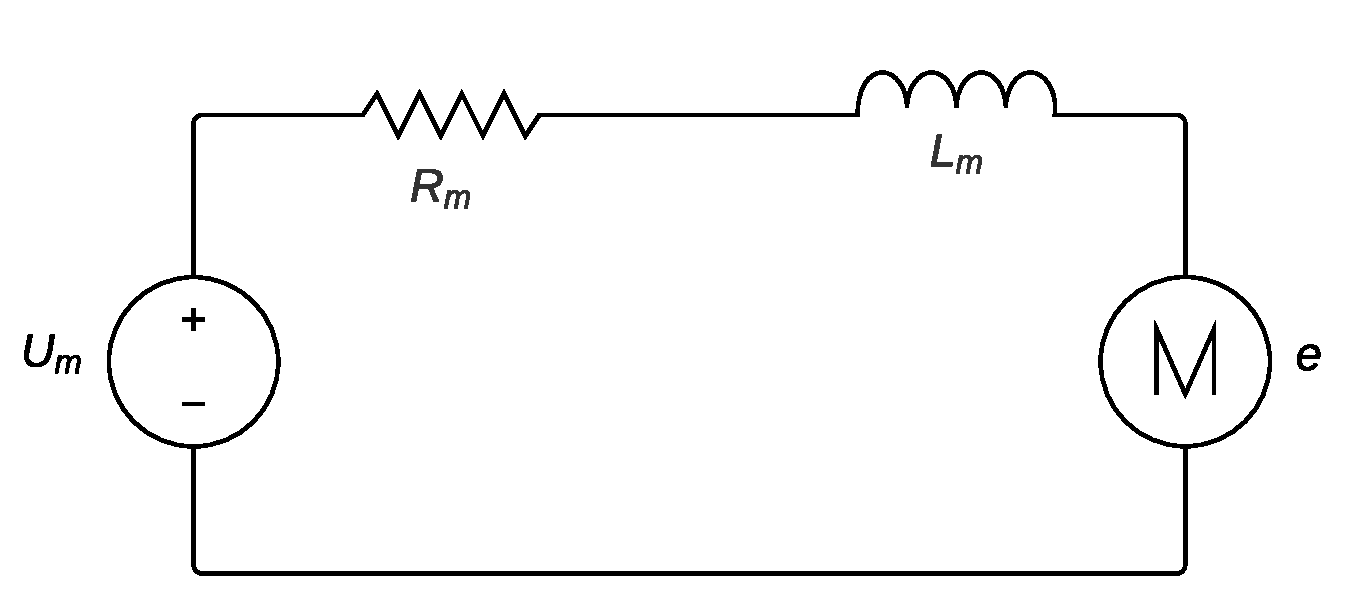
\includegraphics[width=0.7\textwidth]{figures/modeling/Motor/MotorElectricCircuit.pdf} 
 	\caption{Circuit diagram of a DC-motor.}
 	\label{fig:MotorCircuit}
\end{figure}

Using Kirchhoff's voltage law, the electric model of the DC-motor is \autoref{eq:tech_ToA}.
\begin{subequations} \label{eq:tech_ToA}
	\begin{flalign}
		U_m &= R_m \cdot i + L_m \frac{di}{dt} + e \\
		e &= K_e \cdot \omega_m 
	\end{flalign}
\end{subequations}
\startexplain
	\explain{$U_m$ is the voltage output of the generator}{\si{\volt}}
	\explain{$R_m$ is the resistance of the DC-motor}{\si{\ohm}}
	\explain{$L_m$ is the inductance of the DC-motor}{\si{\henry}}
	\explain{$i$ is the current in the DC-motor}{\si{\ampere}}
	\explain{$e$ is the electromotive force}{\si{\volt}}
	\explain{$K_e$ is the motor velocity constant}{\si{\volt\second\per\radian}}
	\explain{$\omega_m$ is the angular velocity of the motor}{\si{\radian\per\second}}
\stopexplain

This is all that's needed for the electrical part to find the model of the motor.

\subsection{Mechanical Model of the Motor}
The mechanical free body diagram of the motor is presented in \autoref{fig:MotorBodyDiagram}.

\begin{figure}[htbp]
	\centering
 	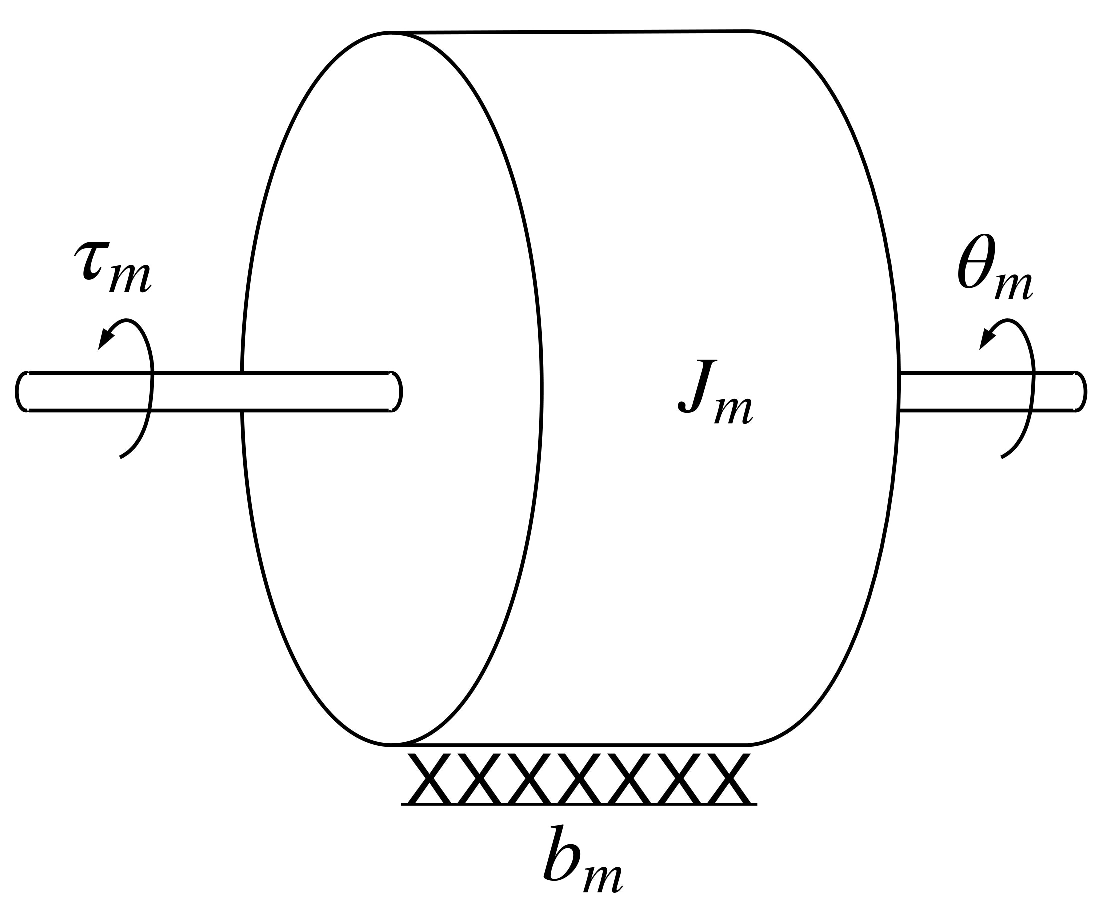
\includegraphics[width=0.4\textwidth]{figures/modeling/Motor/DCMotorMechanic.pdf} 
 	\caption{Free body diagram of a DC-motor.}
 	\label{fig:MotorBodyDiagram}
\end{figure}

From \autoref{fig:MotorBodyDiagram}, the sum of the torques for the mechanical part of the motor is \autoref{eq:MotorMechanical}.

\begin{flalign}
J_{m} \dot{\omega}_{m} = \tau_{m} - \tau_{l} - \tau_{fm} \label{eq:MotorMechanical}
\end{flalign}
\startexplain
	\explain{$J_m$ is the moment of inertia of the motor}{\si{\kilo\gram\meter\squared}}
	%\explain{$\omega_m$ is the angular velocity of the DC-motor}{\si{\radian\per\second}}
	\explain{$\tau_m$ is the torque of the DC-motor}{\si{\newton\meter}}
	\explain{$\tau_l$ is the torque of the load}{\si{\newton\meter}}
	\explain{$\tau_{fm}$ is the torque of the friction}{\si{\newton\meter}}
\stopexplain

The motor's torque and the friction's torque, respectively $\tau_m$ and $\tau_f$, are defined by \autoref{eq:tauLm} while $\tau_l$ is the torque of the gears, $\tau_{gear}$, found in \autoref{sec:torqueGear}.
\begin{subequations}\label{eq:tauLm}
	\begin{flalign}
		&\tau_m = K_t \cdot i  \label{eq:MotorTorque}\\	
		&\tau_{fm} = b_{m}\cdot\omega_{m}	\label{eq:FrictionTorque}
	\end{flalign}
\end{subequations}
\startexplain
	\explain{$K_t$ is the motor torque constant}{\si{\newton\meter\per\ampere}}
	\explain{$b_m$ is the viscous friction coefficient}{\si{\newton\meter\second\per\radian}}
\stopexplain

Inserting \autoref{eq:tauLm} into \autoref{eq:MotorMechanical} gives \autoref{eq:Jm}.
\begin{flalign}
	J_{m} \dot{\omega}_{m} = K_{t}  i - \tau_{gear} - b_{m}  \omega_{m} \label{eq:Jm}
\end{flalign}

The mechanical and electrical model of the motor can now be combined.

\subsection{Combined Model of the Motor}
First the electrical and mechanical equations of the motor are Laplace-transformed in \autoref{eq:MotorLaplace}
\begin{subequations}\label{eq:MotorLaplace}
\begin{flalign}
&U_{m}(s) = R_{m}I(s) + sL_{m} I(s) + K_{e} \Omega_{m}(s) \label{eq:ElectricalLaplace}\\	
&s\cdot J_{m} \Omega_{m}(s) = K_{t} I(s) - \tau_{gear} - B_{m} \Omega_{m}(s) 	\label{eq:MechanicalLaplace}
	\end{flalign}
\end{subequations}

%The current, I(s), is isolated in \autoref{eq:ElectricalLaplace}:
%\begin{equation}
%	I(s)=\frac{U_m(s)-K_e\cdot\Omega(s)}{R_m+sL_m} \addunit{1}
%	\label{eq:MotorCurrent}
%\end{equation}

%Then \autoref{eq:MotorCurrent} is inserted in \autoref{eq:MechanicalLaplace}:
The current, $I(s)$, is isolated and inserted in \autoref{eq:MechanicalLaplace} giving \autoref{eq:Iinserted}.
\begin{flalign}
s\cdot J_{m} \Omega_{m}(s) = K_{t} \frac{U_m(s)-K_e\Omega_{m}(s)}{R_m+sL_m} - \tau_{gear} - B_{m} \Omega_{m}(s)	\label{eq:Iinserted}	
\end{flalign}

\autoref{eq:TaufSimplified} is inserted in \autoref{eq:Iinserted} and rearranged giving \autoref{eq:DCModelYesL}.
\begin{subequations}
\begin{flalign}
&\Omega_m(s)\left(\left(J_m+J_{gear}\right)s+\left(B_m+B_{gear}\right)\right)=K_t\frac{U_m(s)-K_e\Omega_m(s)}{R_m+sL_m} \\
&\Omega_m(s)\left(\left(J_m+J_{gear}\right)L_ms^2+\left(J_m+J_{gear}+\left(B_m+B_{gear}\right)L_m\right)s+\left(B_m+B_{gear}\right)R_m+K_tK_e\right)=K_tU_m(s) \\
\end{flalign}
\end{subequations}

